\subsection{Closed Loop}
\label{sec:closed_loop}
\begin{figure*}
\centering
%\vspace*{-0.3cm}  
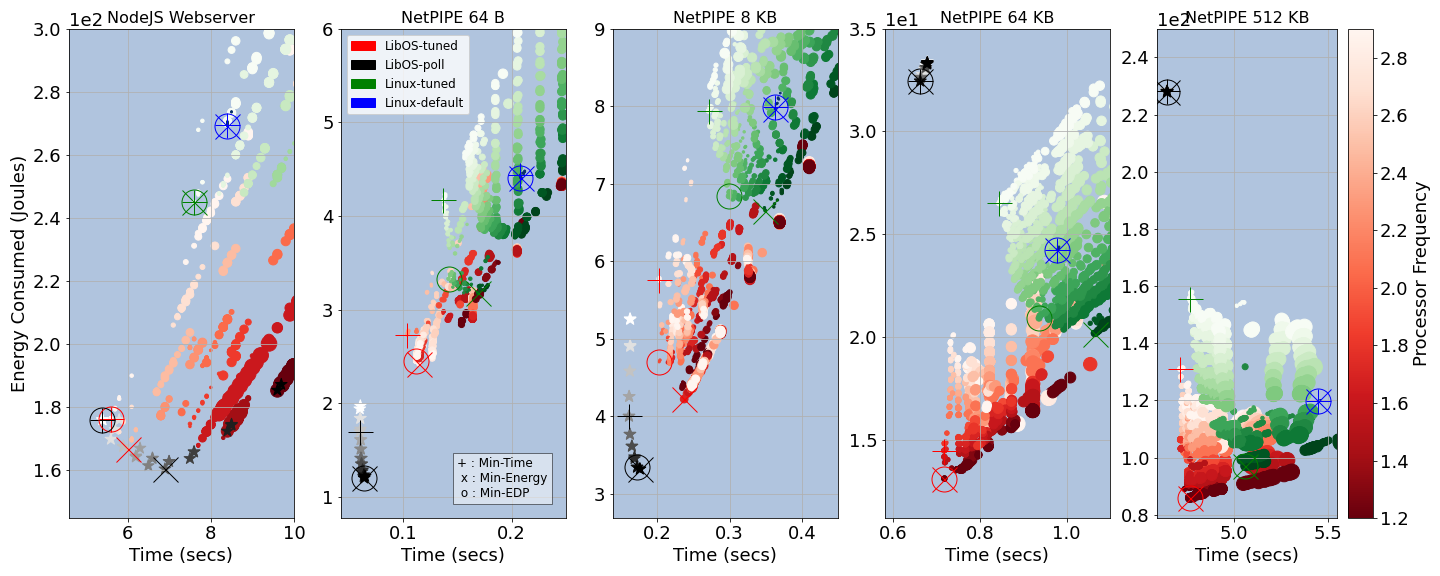
\includegraphics[width=1\textwidth]{figures/closed_loop_overview.png}
\vspace*{-9mm}
\caption[]
%{\small 
{Overview of closed loop experiments: nodejs webserver and netpipe at message sizes 64B, 8KB, 64KB, and 512 KB.
A larger circle equates to slower interrupt delay;
A darker color indicates slowing down the processor;
\textbf{x} indicates lowest energy consumption;
\textbf{+} indicates lowest time spent;
\textbf{o} indicate lowest EDP.
\textbf{Note: X and Y axis are scaled differently to expose structure}}
\label{fig:closed_loop_overview}
\end{figure*}
\begin{figure*}
\centering
%\vspace*{-0.3cm}  
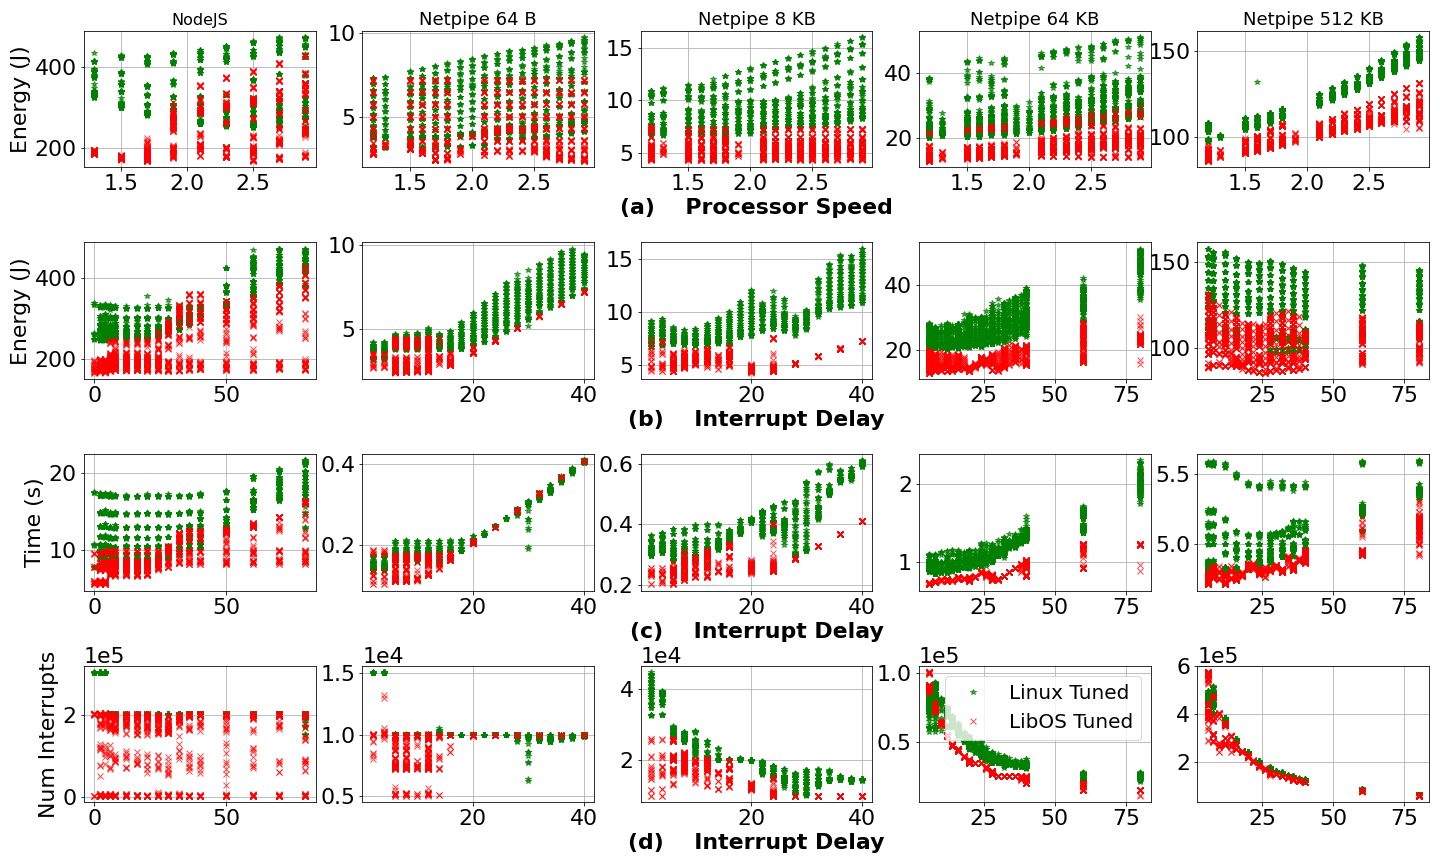
\includegraphics[width=1\textwidth]{figures/closed_detail_1.png}
\vspace*{-9mm}
\caption[]
%{\small 
{Detailed plots of some gathered statistics from the above closed loop experiments.
These plots compare LibOS-tuned and Linux-tuned.
\textbf{Note: X and Y axis are scaled differently to expose structure}}
\label{fig:closed_loop_detail_1}
\end{figure*}
%This approach makes the workloads more predictable and can help smooth out diurnal variations as well~\cite{10.1145/2168836.2168842, 10.1145/2000064.2019527, oldi-study}.
% As pointed out in previous studies of energy proportionality in datacenters, the nature of web-centric applications causes diurnal troughs~\cite{Barroso:2009:DCI:1643608, oldi-study, oldi-pegasus, warehouse-power, energyproportion, WebSearch} and one method with which to increase energy efficiency during these troughs is to maximize the amount of work done, typically under a given energy budget. Figure~\ref{fig:closed_loop_overview} illustrates the set of closed-loop workloads studied in our work, all of the workloads are run in a single core with a single connection, further, they enable us to explore these simple closed-loop examples in detail in settings of computationally intensive (nodejs) and across varying network bandwidth requirements (netpipe). 

Figure~\ref{fig:closed_loop_overview} illustrates the set of closed-loop workloads that we study, all of which are run on a single core with a single connection.
Netpipe~\cite{snell1996netpipe} involves sending messages of identical size between two systems for a fixed number of iterations.
We run Netpipe in a symmetric configuration, whereby the client and server sides run the same software stack and are configured with the same performance parameters. This approach allows us to analyze Netpipe performance precisely, as it eliminates any potential ambiguity in the measurements that may arise from computational differences between the communicating client and server.
Linux runs NetPIPE-3.7.1 while the library OS uses a custom version ported to its interfaces.
We fix the iteration count at 5000 and show results for a range of message sizes \footnote{We found that the 10 GB link is close to saturation when a message of size greater 700 KB is exchanged.}.
As message size increases, the workload becomes more network bound; moreover, Linux suffers an additional memory copy from kernel to userspace compared to the libOS.

NodeJS~\cite{nodejs} consists of a JavaScript HTTP Webserver running inside a nodejs runtime. A single client running the \textit{wrk-4.0.2}~\cite{wrk} benchmark\footnote{We modified \textit{wrk} to place a fixed request load of 100K.} sends web requests to the nodejs server for a fixed period of time. The server responds to each request with a small static payload of size 148 bytes.
Linux runs nodejs-0.10.46, and the library OS runs the same version ported to support bare-metal nodejs by providing OS interfaces that link with the V8~\cite{v8} JavaScript engine and libuv~\cite{libuv}. 

Note that though we use energy-delay-product (EDP) as an energy efficiency measure in our experiments, we refer to it in a different context than that used by the architecture community~\cite{573184,10.1109/40.888701}.
This is because, as datacenter energy use continues to rise~\cite{gupta2020chasing, NLP-energy,warehouse-power,nature1}, traditional metrics such as EDP should be elevated when studying the efficiency of web-centric applications and systems.
Hence we refer to EDP in the closed loop experiments as an energy-efficiency measure that pertains to getting a fixed amount of work done, in contrast to the architecture community which uses EDP as an energy-efficiency measure of instructions.
See the {\larger[4]\textbf{o}} graphical indicator for the setting with best (lowest) EDP.
%% efficiency related to instructions
%% we use efficiency relative to application performance

%We believe these set of workloads will help to simplify the complexity which to compare and contrast the effects of slowing down in the four types of systems listed above.

%\subsubsection{Observation-1: Computationally heavy applications exhibits more performance-energy trade-offs}
%Comparing the nodejs and netpipe workloads in figure~\ref{fig:closed_loop_overview}, one can see the differences in trade-offs as processor is slowed. In netpipe, the \textit{vertical-ness} as the datapoints get darker shows that slowing down the processor does not cause an increase in time, whereas the opposite is shown in the nodejs data.

% MIN-TIME linux_default   1 3.0 8.396 269.4
% MIN-TIME linux_tuned     2 2.9 7.599 244.93

% MIN-TIME linux_default 64 1 3.0 0.21 4.44
% MIN-TIME linux_tuned   64 2 2.9 0.14 4.17

% MIN-TIME linux_default 8192 1 3.0 0.36 7.99
% MIN-TIME linux_tuned   8192 8 2.8 0.27 7.94

% MIN-TIME linux_default 65536 1 3.0 0.98 24.25
% MIN-TIME linux_tuned   65536 8 2.9 0.84 26.5

% MIN-TIME linux_default 524288 1 3.0 5.45 119.77
% MIN-TIME linux_tuned   524288 8 2.9 4.77 155.56

% MIN-TIME ebbrt_tuned   4 2.9 5.6 176.11 986.11
% MIN-TIME ebbrt_poll    0 2.9 5.4 176.01 950.1

% MIN-TIME ebbrt_tuned 64 2 2.3 0.1 2.73 0.28
% MIN-TIME ebbrt_poll  64 0 2.5 0.06 1.7 0.1

% MIN-TIME ebbrt_tuned 8192 6 2.9 0.2 5.76 1.16
% MIN-TIME ebbrt_poll  8192 0 2.1 0.16 4.0 0.64

% MIN-TIME ebbrt_tuned 65536 6 1.7 0.72 14.46 10.35
% MIN-TIME ebbrt_poll  65536 6 1.3 0.66 32.45 21.48

% MIN-TIME ebbrt_tuned 524288 6 2.9 4.72 130.94 617.38
% MIN-TIME ebbrt_poll  524288 6 2.7 4.64 228.13 1059.59



% MIN-EDP linux_default 1 3.0 8.4 269.27 2261.6
% MIN-EDP linux_tuned   2 2.9 7.6 244.93 1861.22

% MIN-EDP linux_default 64 1 3.0 0.21 4.41 0.92
% MIN-EDP linux_tuned   64 2 2.1 0.14 3.33 0.47

% MIN-EDP linux_default 8192 1 3.0 0.36 7.99 2.89
% MIN-EDP linux_tuned   8192 10 2.0 0.3 6.84 2.05

% MIN-EDP linux_default 65536 1 3.0 0.98 24.25 23.72
% MIN-EDP linux_tuned   65536 12 1.8 0.94 20.91 19.57

% MIN-EDP linux_default 524288 1 3.0 5.45 119.77 652.63
% MIN-EDP linux_tuned   524288 28 1.2 5.06 97.04 491.22


% MIN-EDP ebbrt_tuned   4 2.9 5.6 176.11 986.11
% MIN-EDP ebbrt_poll    0 2.9 5.4 175.93 949.67

% MIN-EDP ebbrt_tuned   64 6 2.9 0.11 2.45 0.27
% MIN-EDP ebbrt_poll    64 0 1.2 0.06 1.2 0.08

% MIN-EDP ebbrt_tuned 8192 2 1.9 0.2 4.7 0.95
% MIN-EDP ebbrt_poll  8192 0 1.3 0.17 3.34 0.57

% MIN-EDP ebbrt_tuned 65536 6 1.2 0.72 13.07 9.37
% MIN-EDP ebbrt_poll  65536 6 1.3 0.66 32.45 21.48

% MIN-EDP ebbrt_tuned 524288 26 1.2 4.77 85.94 409.68
% MIN-EDP ebbrt_poll  524288 6 1.5 4.65 227.86 1058.57

% find configurations in which the OS interacts with slowing down to improve both time and energy. 
\subsubsection{Reducing Time to Save Energy}
\label{sec:closed_loop:speedup}
%% relation between quiescent and time to do work
%As discussed in \cref{sec:workflow:closed_loop}, 
Figure~\ref{fig:closed_loop_overview} demonstrates the correlation between minimizing the time needed to finish work and the relevant energy savings.
One mechanism to reduce time across all the closed loop workloads and system types is to speed up interrupt delays (set a low interrupt delay value) as shown in figure~\ref{fig:closed_loop_detail_1}(c).
While slowing down the processor does cause fluctuations in time under each set interrupt delay value, the overall trend is \textit{that low interrupt delay results in lowest overall time}.

By reducing time, one also minimizes energy, as shown in figure~\ref{fig:closed_loop_detail_1}(b). For nodejs and netpipe 64B, we found that setting a low interrupt delay (2$\mu$s) resulted in the lowest EDP, due to the lightweight nature of the payloads themselves (under a single MTU). However, as the payload sizes increase (to 8KB, 64KB, and 512KB), we found the interrupt delay value that yields best EDP also become larger, up to 28$\mu$s at 512 KB. A 10 GbE NIC, assuming no network jitter and switching cost, can transmit at an optimal rate of 1250 bytes/$\mu$s.
\textit{Setting a static interrupt delay value is effectively determining how much payload the software should process in some fixed quantum}. With larger message sizes, one can imagine portions of its payload being transmitted over the wire and processed by software asynchronously. The interrupt delay value that yields best EDP is indicating an optimal configuration with which the software should pace packet processing and save energy by sleeping during the its quiescent periods.

By modulating interrupt delay, Linux-tuned improves its EDP over Linux-default by 21\%-80\%. Due to the OS path length efficiency of the library OS (see figure~\ref{fig:closed_loop_detail_1}(a)), the library OS always uses fewer instructions, even in computationally heavy workloads such as nodejs (7.2\% less).
This efficiency, coupled with a custom interrupt delay, enables libOS-tuned to achieve up to 2X better EDP than Linux-tuned.

%One can also notice the wider variation in time for nodejs in figure~\ref{fig:closed_loop_detail_1}(c), this is mainly the result of greater performance-energy trade-offs that occur in a computationally bound application.

\subsubsection{Trade-offs in Library OS Polling}
\label{sec:closed_loop:poll}
We compare the energy-performance trade-offs between slowing down the processor while the library OS is in a polling loop (LibOS-poll) and slowing down both processor and interrupt delay (LibOS-tuned) otherwise.
For nodejs, LibOS-poll results in a 4\% better (lower) EDP than that of LibOS-tuned. This is due to the nodejs runtime already using an application-level poll to check for new packets.

Interestingly, the difference in EDP for LibOS-poll is quite dramatic as message size increases in Netpipe. With 64B and 8KB message sizes, polling improves EDP by 1.6X and 3X respectively over LibOS-tuned. This is because for smaller payload sizes, getting the work done fastest still results in the lowest energy use.
In some sense, this mirrors the explanation in \cref{sec:closed_loop:speedup}, where the best EDP for smaller payload sizes uses fast interrupt delays (i.e. an interrupt-based poll behavior). At 64KB and 512 KB, the workload becomes more network bound and polling results in worse EDP by up to 2X compared to LibOS-tuned. We find at these larger message sizes sizes, polling only reduced time over LibOS-tuned by around 10\%.
However, energy consumption by polling was over 2X worse, which is indicative that packets spent more time on the wire than in software.
This phenomena suggests the importance of a hybrid strategy that switches between poll and interrupt-driven OS policies as payload size changes in a closed loop setting.

\subsubsection{Slowing Down to Stay Busy}
\label{sec:closed_loop:slowtostaybusy}
Previous works have coined terms such as race-to-idle/ pace-to-idle~\cite{10.1145/2525526.2525854} for alternative energy saving strategies. In both nodejs and Netpipe with message size 64B, we find another interesting effect. In figure~\ref{fig:closed_loop_detail_1}(d); for various interrupt delay values, the total number of interrupts can be lowered by up to 90\%.
Upon closer examination, we find that slowing down of the processor causes this decrease in number of interrupts.

The reason for this behavior in the library OS is described briefly in section~\ref{sec:workflow:osrepproc}:
The physical transmission of OS reply packets by the network driver can occur in asynchrony with the unwinding of the stack back to the nodejs application and then back down to the network receive function to check for new packets.
The slowing down of the processor causes this unwind path to lengthen, potentially increasing the probability that new packets have already arrived ready to be processed by the time it reaches the network receive function.
Therefore, the software is able to skip one or more hardware interrupts (fired on packet receive) in order to effectively stay busy and process this new reply packet.
This scenario only occurs in the library OS due to its run-to-completion nature and suggests that, for such a structurally different OS design, a different energy saving strategy is needed.

%what are configurations where this doesn't occur??
%In the library OS, we find slowing down of the processor results in a new energy efficient state which we term \textit{slow-to-stay-busy}.
% MIN-TIME linux_default 65536 1 3.0 0.98 24.25 23.72
% MIN-TIME linux_tuned 65536 8 2.9 0.84 26.5 22.37
% MIN-TIME ebbrt_tuned 65536 6 1.7 0.72 14.46 10.35
% MIN-TIME ebbrt_poll 65536 6 1.3 0.66 32.45 21.48

% MIN-TIME linux_default 524288 1 3.0 5.45 119.77 652.63
% MIN-TIME linux_tuned 524288 8 2.9 4.77 155.56 741.87
% MIN-TIME ebbrt_tuned 524288 6 2.9 4.72 130.94 617.38
% MIN-TIME ebbrt_poll 524288 6 2.7 4.64 228.13 1059.59



%% Vertical behavior of Netpipe 64 KB and 512 KB??
